\documentclass{article}\usepackage[]{graphicx}\usepackage[]{xcolor}
% maxwidth is the original width if it is less than linewidth
% otherwise use linewidth (to make sure the graphics do not exceed the margin)
\makeatletter
\def\maxwidth{ %
  \ifdim\Gin@nat@width>\linewidth
    \linewidth
  \else
    \Gin@nat@width
  \fi
}
\makeatother

\definecolor{fgcolor}{rgb}{0.345, 0.345, 0.345}
\newcommand{\hlnum}[1]{\textcolor[rgb]{0.686,0.059,0.569}{#1}}%
\newcommand{\hlstr}[1]{\textcolor[rgb]{0.192,0.494,0.8}{#1}}%
\newcommand{\hlcom}[1]{\textcolor[rgb]{0.678,0.584,0.686}{\textit{#1}}}%
\newcommand{\hlopt}[1]{\textcolor[rgb]{0,0,0}{#1}}%
\newcommand{\hlstd}[1]{\textcolor[rgb]{0.345,0.345,0.345}{#1}}%
\newcommand{\hlkwa}[1]{\textcolor[rgb]{0.161,0.373,0.58}{\textbf{#1}}}%
\newcommand{\hlkwb}[1]{\textcolor[rgb]{0.69,0.353,0.396}{#1}}%
\newcommand{\hlkwc}[1]{\textcolor[rgb]{0.333,0.667,0.333}{#1}}%
\newcommand{\hlkwd}[1]{\textcolor[rgb]{0.737,0.353,0.396}{\textbf{#1}}}%
\let\hlipl\hlkwb

\usepackage{framed}
\makeatletter
\newenvironment{kframe}{%
 \def\at@end@of@kframe{}%
 \ifinner\ifhmode%
  \def\at@end@of@kframe{\end{minipage}}%
  \begin{minipage}{\columnwidth}%
 \fi\fi%
 \def\FrameCommand##1{\hskip\@totalleftmargin \hskip-\fboxsep
 \colorbox{shadecolor}{##1}\hskip-\fboxsep
     % There is no \\@totalrightmargin, so:
     \hskip-\linewidth \hskip-\@totalleftmargin \hskip\columnwidth}%
 \MakeFramed {\advance\hsize-\width
   \@totalleftmargin\z@ \linewidth\hsize
   \@setminipage}}%
 {\par\unskip\endMakeFramed%
 \at@end@of@kframe}
\makeatother

\definecolor{shadecolor}{rgb}{.97, .97, .97}
\definecolor{messagecolor}{rgb}{0, 0, 0}
\definecolor{warningcolor}{rgb}{1, 0, 1}
\definecolor{errorcolor}{rgb}{1, 0, 0}
\newenvironment{knitrout}{}{} % an empty environment to be redefined in TeX

\usepackage{alltt}

\usepackage{hyperref}
\usepackage[backend=bibtex, maxnames=10]{biblatex}
\usepackage{xargs}
\usepackage{xcolor}
\usepackage{soul}

\title{Package \textbf{CompSign}}
\author{Lena Morrill}
\date{October 2022}

\setlength{\textwidth}{6.5in}
\setlength{\oddsidemargin}{-0.1in}
\setlength{\textheight}{8.6in}
\setlength{\topmargin}{-0.4in}
\IfFileExists{upquote.sty}{\usepackage{upquote}}{}
\begin{document}

\maketitle

\textbf{CompSign} is a toolkit for differential abundance analysis of mutational signatures using a mixed effects Dirichlet-multinominal model (or simpler variations). The compositional nature of mutational signature exposures has often been overlooked but has important implications, as the analyses must be done in relative terms.

\tableofcontents

\section{Installation}
\texttt{CompSign} can be installed as usual from github:

\begin{knitrout}
\definecolor{shadecolor}{rgb}{0.969, 0.969, 0.969}\color{fgcolor}\begin{kframe}
\begin{alltt}
\hlkwd{library}\hlstd{(devtools)}
\hlstd{devtools}\hlopt{::}\hlkwd{install_github}\hlstd{(}\hlstr{"lm687/CompSign"}\hlstd{)}
\end{alltt}
\end{kframe}
\end{knitrout}

\begin{knitrout}
\definecolor{shadecolor}{rgb}{0.969, 0.969, 0.969}\color{fgcolor}\begin{kframe}
\begin{alltt}
\hlkwd{library}\hlstd{(CompSign)}
\hlkwd{library}\hlstd{(gridExtra)}
\hlkwd{library}\hlstd{(TMB)}
\end{alltt}


{\ttfamily\noindent\color{warningcolor}{\#\# Warning: package 'TMB' was built under R version 4.0.5}}\end{kframe}
\end{knitrout}

\section{Datasets}
\begin{knitrout}
\definecolor{shadecolor}{rgb}{0.969, 0.969, 0.969}\color{fgcolor}\begin{kframe}
\begin{alltt}
\hlcom{## if the folder data/ is not in github}
\hlkwa{for}\hlstd{(i} \hlkwa{in} \hlkwd{list.files}\hlstd{(}\hlstr{"../inst/extdata/"}\hlstd{,} \hlkwc{pattern} \hlstd{=} \hlstr{"*RDA"}\hlstd{,} \hlkwc{full.names} \hlstd{=} \hlnum{TRUE}\hlstd{))\{}\hlkwd{load}\hlstd{(i)\}}
\end{alltt}
\end{kframe}
\end{knitrout}

The package contains the following datasets of exposures of mutational signatures and metadata of the corresponding samples. These datasets are:
\begin{itemize}
\item \verb|PancEndocrine_signaturesMSE|: Signature exposures for early and late mutations, in the PCAWG Panc-Endocrine cohort
\item  \verb|ProstAdenoCA_chrom|: Signature exposures for each chromosome, in the PCAWG Prost-AdenoCA cohort
\end{itemize}

\verb|PancEndocrine_signaturesMSE| is an object of class \verb|sign|

\begin{knitrout}
\definecolor{shadecolor}{rgb}{0.969, 0.969, 0.969}\color{fgcolor}\begin{kframe}
\begin{alltt}
\hlstd{PancEndocrine_signaturesMSE} \hlkwb{=} \hlkwd{load_PCAWG}\hlstd{(}\hlstr{"../inst/extdata/roo/Panc-Endocrine_signaturesMSE_ROO.RDS"}\hlstd{,}
                                         \hlkwc{read_directly} \hlstd{= T,}
                                         \hlkwc{typedata} \hlstd{=} \hlstr{"signaturesMSE"}\hlstd{,} \hlkwc{override_warning_X_Z} \hlstd{= T)}
\end{alltt}
\begin{verbatim}
## [1] "../inst/extdata/roo/Panc-Endocrine_signaturesMSE_ROO.RDS"
## Reading file ../inst/extdata/roo/Panc-Endocrine_signaturesMSE_ROO.RDS
\end{verbatim}
\begin{alltt}
\hlstd{PancEndocrine_signaturesMSE_v2} \hlkwb{=} \hlkwd{load_PCAWG}\hlstd{(}\hlkwc{ct} \hlstd{=} \hlstr{"Panc-Endocrine"}\hlstd{,} \hlkwc{typedata} \hlstd{=} \hlstr{"signaturesMSE"}\hlstd{,} \hlkwc{path_to_data} \hlstd{=} \hlstr{"../inst/extdata/"}\hlstd{,} \hlkwc{load_all_sigs} \hlstd{= F,} \hlkwc{override_warning_X_Z} \hlstd{= T)}
\end{alltt}
\end{kframe}
\end{knitrout}

\begin{knitrout}
\definecolor{shadecolor}{rgb}{0.969, 0.969, 0.969}\color{fgcolor}\begin{kframe}
\begin{alltt}
\hlcom{# PancEndocrine_signaturesMSE}
\end{alltt}
\end{kframe}
\end{knitrout}

\begin{knitrout}
\definecolor{shadecolor}{rgb}{0.969, 0.969, 0.969}\color{fgcolor}\begin{kframe}
\begin{alltt}
\hlkwd{do.call}\hlstd{(}\hlstr{'grid.arrange'}\hlstd{,} \hlkwd{lapply}\hlstd{(}\hlkwd{split_matrix_in_half}\hlstd{(PancEndocrine_signaturesMSE}\hlopt{$}\hlstd{Y),} \hlkwa{function}\hlstd{(}\hlkwc{i}\hlstd{)} \hlkwd{createBarplot}\hlstd{(}\hlkwd{normalise_rw}\hlstd{(i),} \hlkwc{remove_labels} \hlstd{= T)))}
\end{alltt}


{\ttfamily\noindent\itshape\color{messagecolor}{\#\# Loading required package: reshape2}}

{\ttfamily\noindent\itshape\color{messagecolor}{\#\# Loading required package: ggplot2}}

{\ttfamily\noindent\color{warningcolor}{\#\# Warning: package 'RColorBrewer' was built under R version 4.0.5}}\begin{verbatim}
## Creating plot... it might take some time if the data are large. Number of samples: 70
## Creating plot... it might take some time if the data are large. Number of samples: 70
\end{verbatim}
\end{kframe}
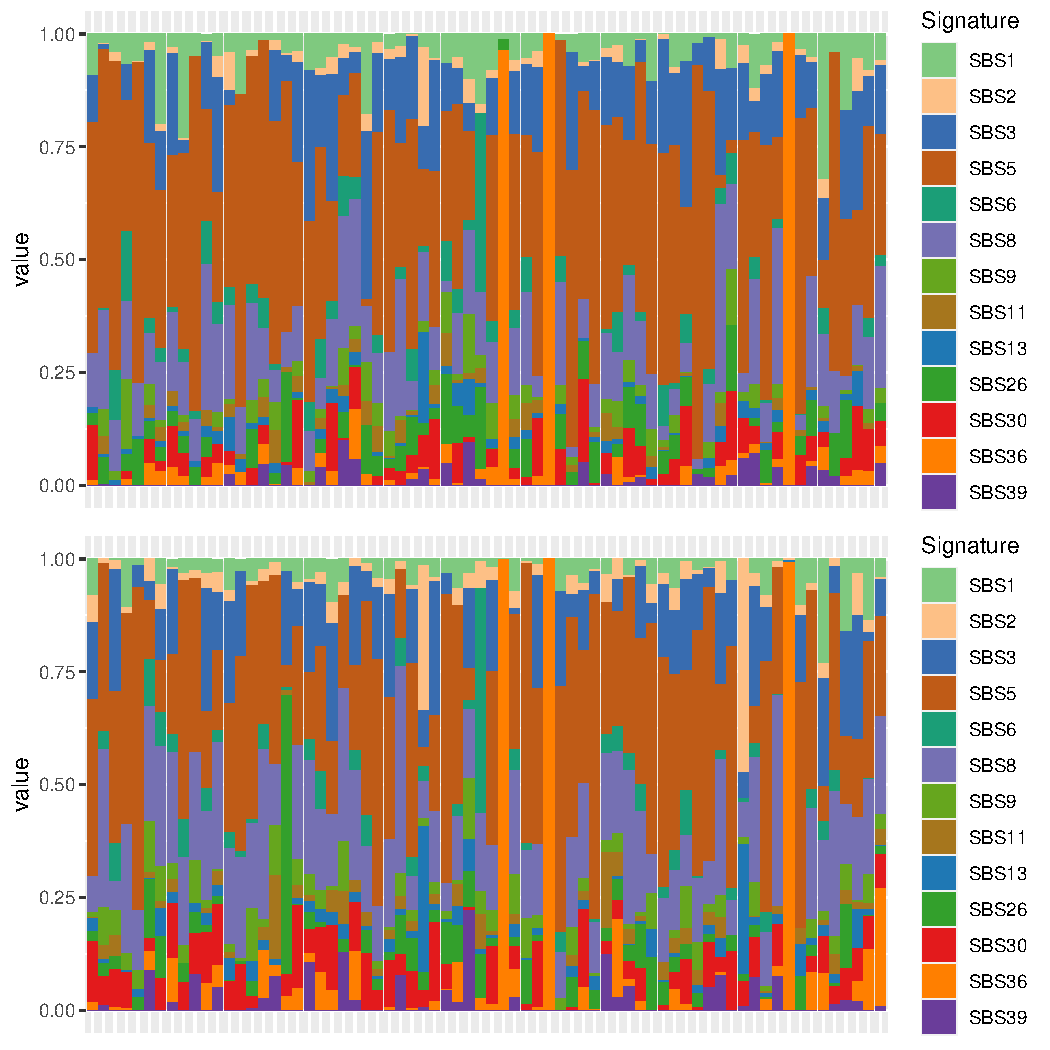
\includegraphics[width=\maxwidth]{figure/unnamed-chunk-4-1} 
\end{knitrout}

\begin{knitrout}
\definecolor{shadecolor}{rgb}{0.969, 0.969, 0.969}\color{fgcolor}\begin{kframe}
\begin{alltt}
\hlkwd{createBarplot}\hlstd{(}\hlkwd{normalise_rw}\hlstd{(}\hlkwd{non_duplicated_rows}\hlstd{(PancEndocrine_signaturesMSE}\hlopt{$}\hlstd{Y)),}
              \hlkwc{order_labels} \hlstd{=} \hlkwd{names}\hlstd{(}\hlkwd{sort}\hlstd{(}\hlkwd{non_duplicated_rows}\hlstd{(PancEndocrine_signaturesMSE}\hlopt{$}\hlstd{Y)[,}\hlstr{'SBS3'}\hlstd{],}
                                        \hlkwc{decreasing} \hlstd{= F)),} \hlkwc{remove_labels}\hlstd{=T)}\hlopt{+}\hlkwd{ggtitle}\hlstd{(}\hlstr{'Sorted by SBS3'}\hlstd{)}
\end{alltt}
\begin{verbatim}
## Creating plot... it might take some time if the data are large. Number of samples: 140
\end{verbatim}
\end{kframe}
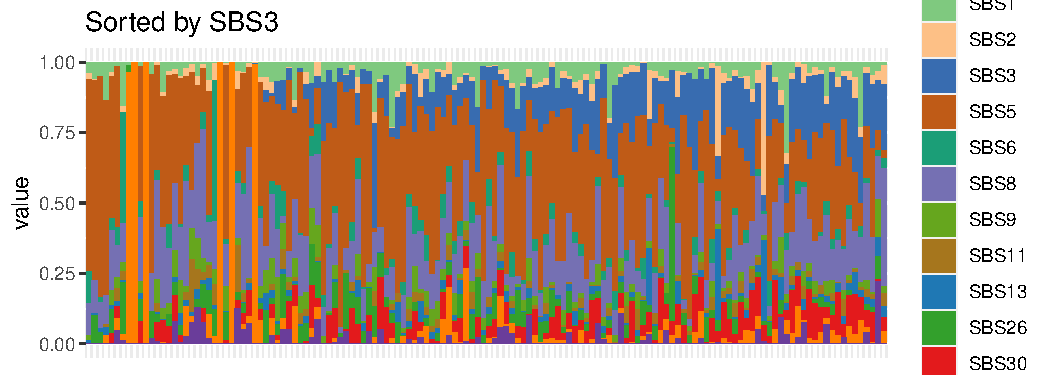
\includegraphics[width=\maxwidth]{figure/panc-endocrine2-1} 
\end{knitrout}

\begin{knitrout}
\definecolor{shadecolor}{rgb}{0.969, 0.969, 0.969}\color{fgcolor}\begin{kframe}
\begin{alltt}
\hlstd{fullDM_no_small_sigs} \hlkwb{<-} \hlkwd{wrapper_run_TMB}\hlstd{(}\hlkwc{object} \hlstd{=} \hlkwd{give_subset_sigs_TMBobj}\hlstd{(PancEndocrine_signaturesMSE,}
                           \hlkwc{sigs_to_remove} \hlstd{=} \hlkwd{c}\hlstd{(}\hlstr{'SBS13'}\hlstd{,} \hlstr{'SBS17a'}\hlstd{,} \hlstr{'SBS17b'}\hlstd{,} \hlstr{'SBS30'}\hlstd{)),}
                                        \hlkwc{model} \hlstd{=} \hlstr{"fullRE_DM"}\hlstd{,} \hlkwc{use_nlminb}\hlstd{=T,} \hlkwc{smart_init_vals}\hlstd{=F)}
\end{alltt}


{\ttfamily\noindent\bfseries\color{errorcolor}{\#\# Error in .Call("{}getParameterOrder"{}, data, parameters, new.env(), NULL, : "{}getParameterOrder"{} not available for .Call() for package "{}fullRE\_ME\_dirichletmultinomial"{}}}\end{kframe}
\end{knitrout}


\end{document}
% ProstAdenoCA_chrom = readRDS("../inst/extdata/roo/ProstAdenoCA_chrom.RDS")
